\documentclass[11pt]{article}
\usepackage[catalan]{babel}
\usepackage{graphicx}
\usepackage[margin=1in]{geometry}
\usepackage{fancyhdr}
\usepackage{lipsum}
\usepackage{tikz}
\usepackage[hidelinks]{hyperref}
\pagestyle{fancy}

\title{\bfseries\Huge OrionWay}
\author{RLP - Grup 5}

\rhead{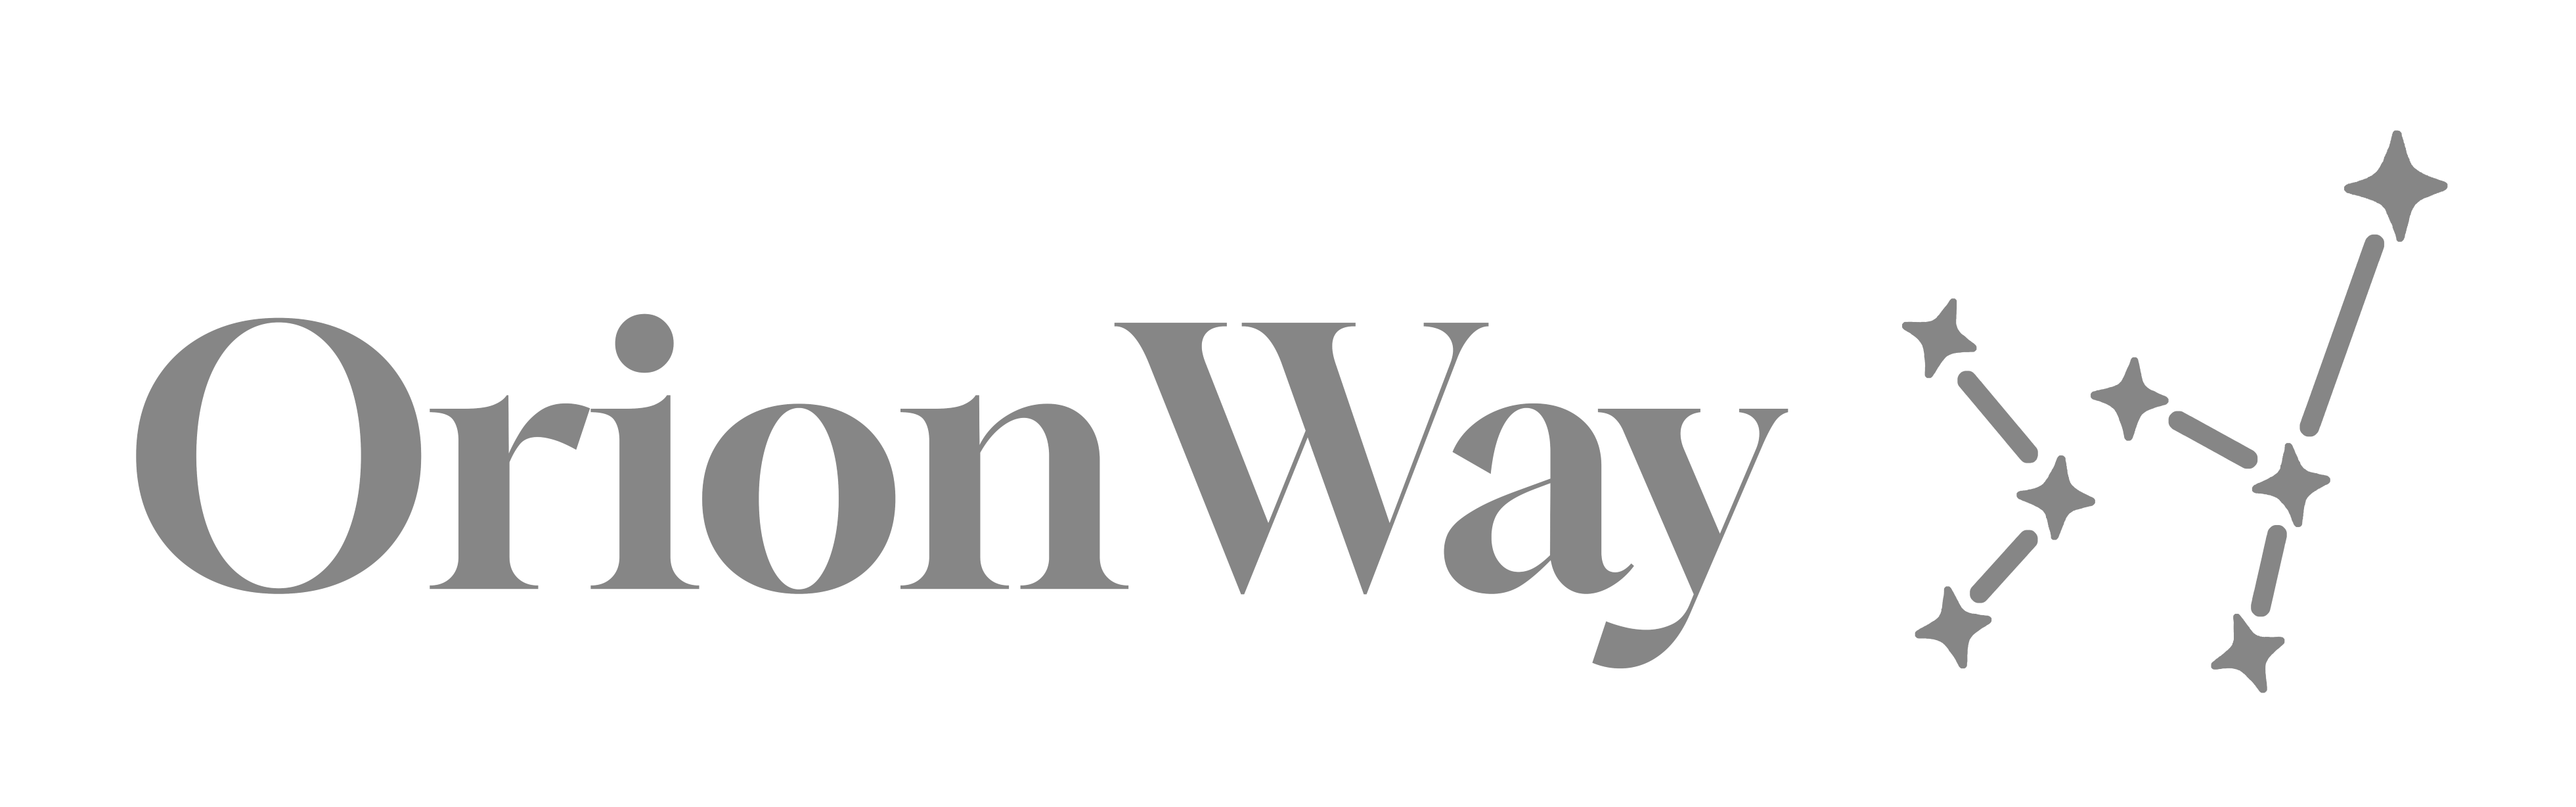
\includegraphics[height=0.08\linewidth]{../orionway_transparent}}
\renewcommand{\headrulewidth}{0pt}
\renewcommand{\footrulewidth}{0pt}
\setlength{\headsep}{1.5cm}

\usetikzlibrary{er,positioning}

\begin{document}
	
	%\maketitle
	%\begin{abstract}
	%\end{abstract}
	%\newpage
	\begin{center}
		\vspace*{0.25cm}
		{\Huge \bfseries Disseny inicial}\\[0.5cm]
		{\Large RLP - Grup 5}\\[0.25cm]
		\today
	\end{center}
	
	\section*{Introducció}
	OrionWay és un robot dissenyat per oferir assistència a persones amb discapacitat visual. Aquest ajudarà aquestes persones a desplaçar-se pel carrer evitant els perills existents (barreres, persones, travessar passos de zebra...).
	
	L'usuari estarà en contacte amb el robot durant els trajectes, notant quan aquest es desvia, dirigint-lo manualment, o inclús utilitzant-lo per a identificar objectes desconeguts.
	
	\section*{Especificació}
	Les funcionalitats que tindrà OrionWay seran:
	\begin{itemize}
		\item \hyperlink{sec:a}{Detecció i reacció a obstacles immediats}
		\item \hyperlink{sec:b}{Detecció i reacció a passos de zebra amb semàfors}
		\item \hyperlink{sec:c}{Dirigir manualment el robot en qualsevol moment}
		\item \hyperlink{sec:d}{Reconeixement d'objectes i resposta per veu}
		\item \hyperlink{sec:e}{Apropament automàtic cap a l'usuari en entorns tancats}
		\item \textit{Guiatge cap a ubicacions marcades en un mapa.}
	\end{itemize}
	
	\hypertarget{sec:a}{}
	\subsection*{Detecció i reacció a obstacles immediats}
	Mitjançant els tres sensors d'ultrasons situats al cos del robot i connectats a la placa Arduino, aquest serà capaç de detectar elements propers i modificar la trajectòria dels motors per tal d'esquivar-los. Ha de ser una funcionalitat molt ràpida i eficient, per tal d'aconseguir el millor temps de reacció.
	
	\hypertarget{sec:b}{}
	\subsection*{Detecció i reacció a passos de zebra amb semàfors}
	Mitjançant la càmera i un model de visió per computador, podrem saber l'orientació dels passos de zebra propers, a més de detectar si els seus semàfors es troben en verd o en vermell. Això permetrà encarar el pas de zebra i creuar-lo quan pertoqui, evitant el perill.
	
	\hypertarget{sec:c}{}
	\subsection*{Dirigir manualment el robot en qualsevol moment}
	En qualsevol moment dins el guiatge del robot, l'usuari podrà prémer els botons del mànec per a forçar manualment girs a la dreta o a l'esquerra. \textbf{IMPORTANT:} Aquesta funcionalitat no tindrà més prioritat que les dues funcionalitats anteriors, és a dir, si a l'esquerra del robot es troba un obstacle immediat o un pas de zebra amb semàfor en vermell, el robot es detindrà.
	
	\hypertarget{sec:d}{}
	\subsection*{Reconeixement d'objectes i resposta per veu}
	En qualsevol moment, l'usuari podrà preguntar al robot què subjecta a la seva mà mitjançant els botons situats al mànec. És a dir, utilitzant la càmera, el robot es detindrà, girarà la càmera, farà un reconeixement per imatge de l'objecte que l'usuari li mostri, i s'utilitzarà l'altaveu per a dir la resposta. 
	
	\hypertarget{sec:e}{}
	\subsection*{Apropament automàtic cap a l'usuari en entorns tancats}
	En situacions en què el robot té visió de l'usuari en un entorn tancat, aquest podrà ser cridat per l'usuari picant dues vegades de mans. Quan això succeeixi, el robot farà fotografies en tots els seus angles i detectarà la direcció on es troba l'usuari. Aleshores, utilitzant els sensors d'ultrasons, navegarà fins a l'usuari desplaçant-se al voltant dels obstacles que podrà trobar.
	
\end{document}
